% Created 2016-04-15 Fri 17:17
\documentclass[9pt,b5paper]{article}
\usepackage{graphicx}
\usepackage{xcolor}
\usepackage{xeCJK}
\setCJKmainfont{SimSun}
\usepackage{longtable}
\usepackage{float}
\usepackage{textcomp}
\usepackage{geometry}
\geometry{left=0cm,right=0cm,top=0cm,bottom=0cm}
\usepackage{multirow}
\usepackage{multicol}
\usepackage{listings}
\usepackage{algorithm}
\usepackage{algorithmic}
\usepackage{latexsym}
\usepackage{natbib}
\usepackage{fancyhdr}
\usepackage[xetex,colorlinks=true,CJKbookmarks=true,linkcolor=blue,urlcolor=blue,menucolor=blue]{hyperref}


\lstset{language=c++,numbers=left,numberstyle=\tiny,basicstyle=\ttfamily\small,tabsize=4,frame=none,escapeinside=``,extendedchars=false,keywordstyle=\color{blue!70},commentstyle=\color{red!55!green!55!blue!55!},rulesepcolor=\color{red!20!green!20!blue!20!}}
\author{deepwaterooo}
\date{\today}
\title{Tetris - Basic Implementation Practice for Android}
\hypersetup{
  pdfkeywords={},
  pdfsubject={},
  pdfcreator={Emacs 24.3.1 (Org mode 8.2.7c)}}
\begin{document}

\maketitle
\tableofcontents


\section{Better version, pretty good}
\label{sec-1}
\begin{itemize}
\item OpenGL 3D version status: 
\begin{itemize}
\item basic Necessary changed has been made, but due to lack of necessary informations, debugging for game flow becomes kind of difficult.
\item working on configuring Android studio environment, and configuring debugging tools so that I could potentially get more information for debugging.
\item will update on Sunday evening for studio version.
\item 
\item working slowing step-by-step to get app run without crashing down, getting familiar with app flow \& different opengl modules, many bugs on the ways need to be fixed before onto those matrix.
\item but will get them done. I will.
\item 
\item game layout structure:
\end{itemize}
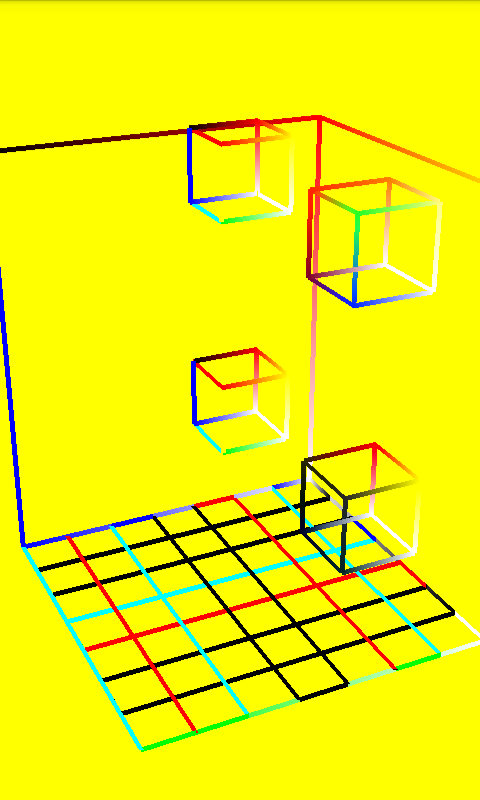
\includegraphics[width=.9\linewidth]{./Screenshot_2016-04-07-11-58-28.png}
\item most challenge part for tonight, matrix translations \& rotations\ldots{}.will continue work on it tonight
\item 
\item a video for this Tetris game can be directly watched at \url{https://www.youtube.com/watch?v=Ht4NOrEUtFk}
\item A video for the previous DrawingFun Android App can be watched at \url{https://www.youtube.com/watch?v=YV78Tk5--5M} , or by searching \textbf{deepwaterooo Wang}.
\end{itemize}

\section{References}
\label{sec-2}
\subsection{Activity.runOnUiThread()}
\label{sec-2-1}
\begin{itemize}
\item \url{http://stackvoid.com/introduction-to-Message-Handler-in-Android/}
\item \url{http://m.oschina.net/blog/97619}
\item 
\end{itemize}

\subsection{3D design}
\label{sec-2-2}
\begin{itemize}
\item c++ version: \url{https://github.com/matachi/tetris-cpp}
\item refer 6 \url{http://www.oschina.net/question/614942_62370}
\item \url{http://www.oschina.net/question/565065_67280}
\item triangle: \url{http://stackoverflow.com/questions/9945321/triangle-opengl-in-android}
\item \url{https://gist.github.com/SebastianJay/3316001}
\item 射线拾取: \url{http://itdocument.com/479827008/}
\item 旋转及手势: \url{http://vaero.blog.51cto.com/4350852/790620}
\item 2 \url{http://vaero.blog.51cto.com/4350852/790637}
\item \url{http://www.lai18.com/content/951343.html}
\item opengl选择与反馈: \url{http://zhidao.baidu.com/question/496046750245095004.html}
\item \url{http://wenku.baidu.com/view/58190d1efad6195f312ba6f7.html}
\item c++ \url{http://blog.csdn.net/u010223072/article/details/45369075}
\item \url{http://codercdy.com/2015/06/17/openglxue-xi-bi-ji-xuan-ze-he-fan-kui/}
\item \url{https://books.google.com/books?id=u6EHM_OzaFQC&pg=PA1987&lpg=PA1987&dq=opengl\%E9\%80\%89\%E6\%8B\%A9\%E4\%B8\%8E\%E5\%8F\%8D\%E9\%A6\%88&source=bl&ots=L9Y66QSEhu&sig=f1h_RadXRDFsa9L5IY430HGTG34&hl=en&sa=X&ved=0ahUKEwjA6vTRo_jLAhVH3mMKHQIXBxYQ6AEIPDAE#v=onepage&q=opengl\%E9\%80\%89\%E6\%8B\%A9\%E4\%B8\%8E\%E5\%8F\%8D\%E9\%A6\%88&f=false}
\item c++ codes: \url{http://dev.gameres.com/program/Visual/3D/Selection.htm}
\item 画线: c++ \url{http://www.programgo.com/article/43724048060/}
\item draw line: \url{http://www.linuxidc.com/Linux/2011-09/42307p3.htm}
\item \url{http://stackoverflow.com/questions/9217702/open-gl-es-2-0-drawing-a-simple-line}
\item 距阵变换: \url{http://www.cnblogs.com/caster99/p/4780984.html}
\item \url{http://www.flakor.cn/2014-05-15-384.html}
\item shader util: \url{http://blog.csdn.net/shulianghan/article/details/17020359}
\item 详解距阵变换:\url{http://www.cnblogs.com/kesalin/archive/2012/12/06/3D_math.html}
\item \url{http://mail.cfanz.cn/index.php?c=article&a=read&id=270244}
\item one example: \url{http://www.apkbus.com/blog-99192-39498.html}
\item ex2 for shader matrix: \url{http://www.voidcn.com/blog/peanut__love/article/p-2891341.html}
\item 西蒙iPhone-OpenGL ES 中文教程专题: \url{http://www.cocoachina.com/special/2010/0126/404.html}
\item 运动: \url{http://www.cocoachina.com/bbs/read.php?tid-7601-fpage-10.html}
\item 
\item 距阵: \url{http://blog.csdn.net/wangdingqiaoit/article/details/39010077}
\item \url{http://blog.csdn.net/popy007/article/details/5120158} UNV
\item \url{http://www.tqcto.com/article/mobile/23873.html} eye
\item \url{http://blog.csdn.net/wangdingqiaoit/article/details/39937019}
\item \url{https://developer.apple.com/library/ios/documentation/3DDrawing/Conceptual/OpenGLES_ProgrammingGuide/Introduction/Introduction.html}
\item \url{http://blog.csdn.net/shulianghan/article/details/46680803}
\item rotation: \url{http://stackoverflow.com/questions/13480043/opengl-es-android-matrix-transformations}
\item glsl example: \url{http://cse.csusb.edu/tongyu/courses/cs520/notes/android-es2.php}
\item shader parser: \url{http://stackoverflow.com/questions/19452240/opengl-glsl-void-parse-error-on-vertex-shader}
\item separate file: \url{http://stackoverflow.com/questions/30345816/splitting-a-text-file-into-multiple-files-by-specific-character-sequence}
\item 
\item 
\item 
\item 
\end{itemize}

\subsection{GLSurfaceView}
\label{sec-2-3}
\begin{itemize}
\item opengl: \url{http://androidblog.reindustries.com/a-real-open-gl-es-2-0-2d-tutorial-part-1/}
\item Graphics architecture: \url{https://source.android.com/devices/graphics/architecture.html}
\item \url{http://stackoverflow.com/questions/5169338/android-deciding-between-surfaceview-and-opengl-glsurfaceview}
\item \textbf{引路蜂} better: \url{http://blog.csdn.net/mapdigit/article/details/7526556}
\item 真正的3D图形: \url{http://www.imobilebbs.com/wordpress/archives/1554}
\item a Cube: \url{http://www.oschina.net/question/4873_28325}
\item modification: \url{https://github.com/googleglass/gdk-apidemo-sample/blob/master/app/src/main/java/com/google/android/glass/sample/apidemo/opengl/Cube.java}
\item Android OpenGL ES 简明开发教程小结: \url{http://www.imobilebbs.com/wordpress/archives/1583}
\item 
\item 
\item 

\item \url{http://hellosure.github.io/android/2015/06/01/android-glsurfaceview/}
\item \url{http://ju.outofmemory.cn/entry/172850}
\item 画图: \url{http://www.mobile-open.com/2015/81568.html}
\item \url{http://tangzm.com/blog/?p=20}
\item \url{http://www.apkbus.com/blog-99192-39584.html}
\item onDrawFrame intro: \url{http://www.jayway.com/2009/12/03/opengl-es-tutorial-for-android-part-i/}
\item failed: \url{http://stackoverflow.com/questions/28711850/android-opengl-how-to-draw-a-rectangle}
\item onTouchEvent: \url{http://blog.csdn.net/niu_gao/article/details/8673662}
\item volatile \url{http://www.voidcn.com/blog/fanfanxiaozu/article/p-3668133.html}
\item \url{http://mobile.51cto.com/aengine-437172.htm}
\item OpenGLES related: \url{http://stackoverflow.com/questions/9945321/triangle-opengl-in-android}
\item OpenGL ES 2.0 Sample Code: \url{http://androidbook.com/item/4254}
\item intros:详解 \url{http://blog.csdn.net/niu_gao/article/details/7566297}
\item 画线: \url{http://www.cnblogs.com/lhxin/archive/2012/06/01/2530828.html}
\item \url{http://bbs.9ria.com/thread-201740-1-1.html}
\item \url{http://imgtec.eetrend.com/blog/5078}
\item draw a ball \url{http://shikezhi.com/html/2015/android_1022/561912.html}
\item for Board c++: \url{http://www.jiancool.com/article/24471349949/}
\item possible? \url{http://code1.okbase.net/codefile/CCFormatter.java_2015072733469_393.htm}
\item \url{http://www.mobile-open.com/2015/80379.html}
\end{itemize}

\subsection{eventQueue vs SurfaceView threads}
\label{sec-2-4}
\begin{itemize}
\item Deeper summary, android graphics architecture: \url{http://hukai.me/android-deeper-graphics-architecture/}
\item 2 threads, load, read, \url{http://blog.csdn.net/hellogv/article/details/5986835}
\end{itemize}
\subsection{Canvas Path subclass}
\label{sec-2-5}
\begin{itemize}
\item how to define drawLine to be drawShapes?
\end{itemize}
\subsection{SurfaceView}
\label{sec-2-6}
\begin{itemize}
\item Surface runnable \url{http://android.okhelp.cz/surfaceview-implements-runnable-android-code/}
\item Example: \url{http://technicalsearch.iteye.com/blog/1967616}
\item \url{http://www.jcodecraeer.com/a/anzhuokaifa/androidkaifa/2012/1201/656.html}
\item Event Queue: \url{http://www.leestorm.com/post/17.html}
\item lockCanvas(Rect小区) \url{http://blog.csdn.net/alexander_xfl/article/details/13000347}
\item example: \url{http://fanli7.net/a/JAVAbiancheng/ANT/20120424/160203.html}
\item MotionEvent: \url{http://android.jobbole.com/82072/}
\item surfaceview双缓冲: \url{http://blog.csdn.net/cnbloger/article/details/7404485}
\item sth worth try: \url{http://www.lxway.com/969295592.htm}
\item Dont Understand: \url{http://blog.sina.com.cn/s/blog_5a6f39cf01012rtv.html}
\item tried: \url{http://bbs.csdn.net/topics/370074255} drawBitmap 2 canvas
\item slightly complicated: \url{http://www.lxway.com/148606691.htm}
\item slightly complicated: \url{http://www.lxway.com/186948856.htm}
\end{itemize}

\subsection{gestures}
\label{sec-2-7}
\begin{itemize}
\item \url{http://www.cnblogs.com/akira90/archive/2013/03/10/2952886.html}
\item Android 触摸手势基础 官方文档概览: \url{http://www.lxway.com/445554926.htm}
\item 手势: \url{http://wiki.jikexueyuan.com/project/material-design/patterns/gestures.html}
\item \url{http://www.lxway.com/601620614.htm}
\item \url{http://www.lxway.com/282219004.htm}
\item \url{http://www.lxway.com/906451412.htm}
\item \url{http://www.lxway.com/146619692.htm}
\item \url{http://www.lxway.com/4420294641.htm}
\item \url{http://www.lxway.com/155059816.htm}
\item \url{http://www.lxway.com/4019928952.htm}
\item 例子: \url{http://bbs.chinaunix.net/thread-3634477-1-1.html}
\item 例子: \url{http://www.bestappsmarket.com/p/app?appId=1192877&title=tetris-\%E4\%BF\%84\%E7\%BD\%97\%E6\%96\%AF\%E6\%96\%B9\%E5\%9D\%97}
\item 例子: \url{http://bbs.chinaunix.net/thread-3634477-1-1.html}

\item iTetris: \url{http://searchapp.soft4fun.net/article/information/iTetris\%20\%E4\%BF\%84\%E7\%BD\%97\%E6\%96\%AF\%E6\%96\%B9\%E5\%9D\%97/313319}
\item left right: \url{http://www.jb51.net/article/77028.htm}
\item AI: \url{http://www.cnblogs.com/youngshall/archive/2009/03/24/1420682.html}
\item 
\item 3/11/2016 Friday
\item \url{https://github.com/Almeros/android-gesture-detectors} mac
\item \url{http://www.jcodecraeer.com/a/anzhuokaifa/androidkaifa/2015/0211/2467.html}
\item \url{http://www.hejun.biz/81.html}
\item \url{http://www.jb51.net/article/38166.htm}
\item \url{http://www.jb51.net/article/37717.htm}
\item \url{http://mobile.51cto.com/aprogram-394841.htm}

\item TetrisBattle特殊轉入教學(Z S J L I)
\begin{itemize}
\item \url{https://www.youtube.com/watch?v=zW6Gp_7jl9I}
\end{itemize}
\item 推箱子: 第11章 Android游戏开发视频教程 益智游戏——推箱子
\begin{itemize}
\item \url{https://www.youtube.com/watch?v=glzxII1-P0A} 2.5D
\end{itemize}
\item 祖码游戏的设计与实现
\end{itemize}
% Emacs 24.3.1 (Org mode 8.2.7c)
\end{document}